\documentclass[11pt]{article}

\usepackage{array}
\usepackage{clrscode3e}
\usepackage{amsmath}
\usepackage{kbordermatrix}
\usepackage{mathtools}
\usepackage{cite}
\usepackage{hyperref}
\usepackage{rotating}
\usepackage{svg}
\usepackage{pdfpages}

\newcommand{\defeq}{\vcentcolon=}
\newcommand{\eqdef}{=\vcentcolon}

\setlength{\parindent}{0em}
\setlength{\parskip}{1em}

\begin{document}

\title{Efficient Calculation of Polynomial and Interaction Features on Sparse Matrices}
\author{
  Andrew Nystrom\\
  \texttt{awnystrom@gmail.com}
  \and
  John Hughes\\
  \texttt{jfh@cs.brown.edu}
}
\date{}

\maketitle

\begin{abstract}%   <- trailing '%' for backward compatibility of .sty file
We give an algorithm to efficiently calculate second degree polynomial or interaction features for a sparse matrix.
The algorithm has average time complexity that decreases quadratically with respect to the density of the matrix, which
is a large improvement over the naive approach. It also allows for the matrix to remain in sparse form, reducing memory demands.
We apply the method to several real datasets and give both analytical and empirical comparisons with the
naive approach. The work also gives a generalizable method for creating algorithms for higher orders of polynomials.
\end{abstract}

\section{Introduction}
When performing a modeling task, one is often faced with a non-linearly separable problem,
or is attempting to predict a target that is a non-linear combination of the variables at one's disposal.
There are several general classes of methods for dealing with these situations: kernel methods, 
high variance models, and input transformations.

Of the possible types of input transformations one
might apply, a widely used method is the polynomial transformation, which is defined as 
all products of all combinations with replacement of $k$ components of a $D$ dimensional row vector $\vec{x}$ (assuming row-wise instance representation), where $k$ is the degree of the polynomial.
In the case of $k=2$, the following set of polynomial features are augmented to each $\vec{x}_i$:

\begin{equation*}
\{x_a \cdot x_b : a, b \in \{0,1,..., D-1\} \land a \le b\}
\end{equation*}

which results in $\binom{D+1}{D-1} = \frac{D^2+D}{2}$ additional features, so the generation of 
these features for a matrix of size $N \times D$ has a time complexity of $O(ND^2)$. In the general case of degree $k$, there 
are $\binom{D+k-1}{D-1}$ polynomial features and the time complexity is $O(ND^k)$.

To help visualize what second degree polynomial features are capable of in a machine learning paradigm,
we trained a linear classifier (logistic regression) on four different datasets and show their decision
boundaries (figure \eqref{fig:boundaries} on page \pageref{fig:boundaries}) with and without polynomial features, along with their accuracy on a holdout set. We compare
these to an RBF SVM via scikit-learn\footnote{\url{http://scikit-learn.org/stable/modules/generated/sklearn.svm.SVC.html}} 
and gradient boosted decision trees via the xgboost package\footnote{\url{https://github.com/dmlc/xgboost/}}.

\begin{sidewaysfigure}
    \centering
    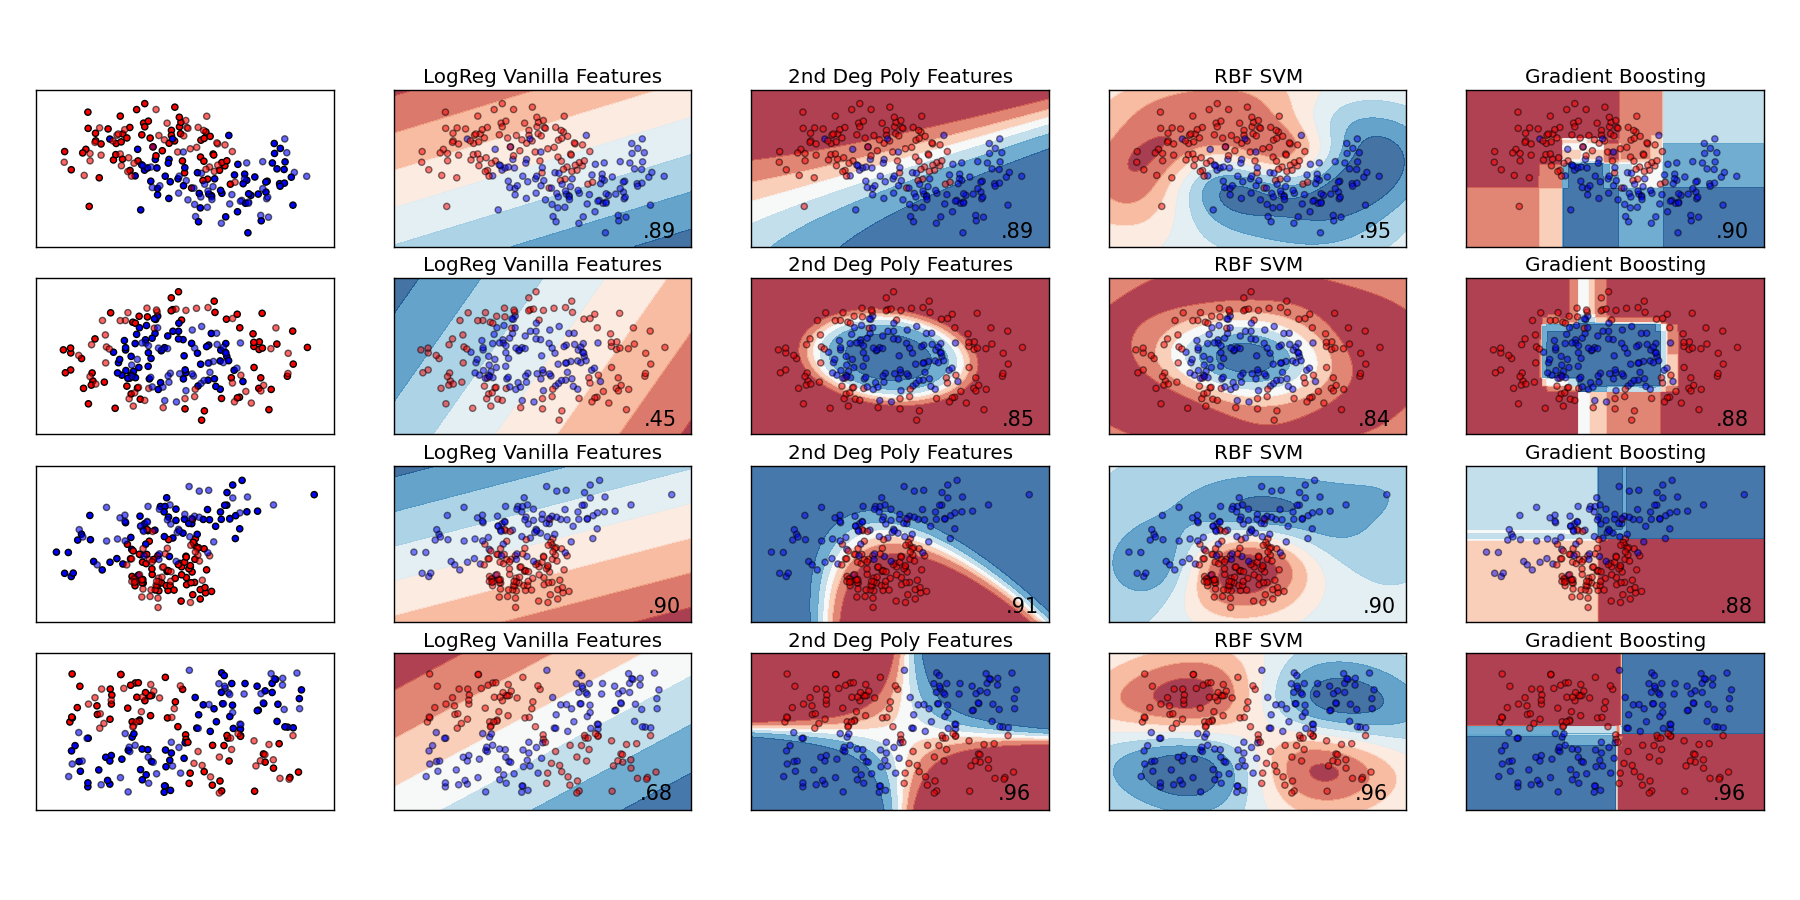
\includegraphics[scale=0.5]{classifier_boundaries.png}
    \caption{Decision boundaries for four classifier types on four different datasets. The darker the color, the more certain the decision.
             The plain dataset is shown in the first column. Each other column is a type of classifier applied to that dataset. The classifier
             types are logistic regression, logistic regression with second degree polynomial features, RBF SVM, and gradient boosting with decision trees.
             The accuracy of each model is shown in the bottom right corner of that model's subplot.}
    \label{fig:boundaries}
\end{sidewaysfigure}

%Same as above, but in vector graphic form. Use this in the final.
%\begin{sidewaysfigure}
%    \centering
%    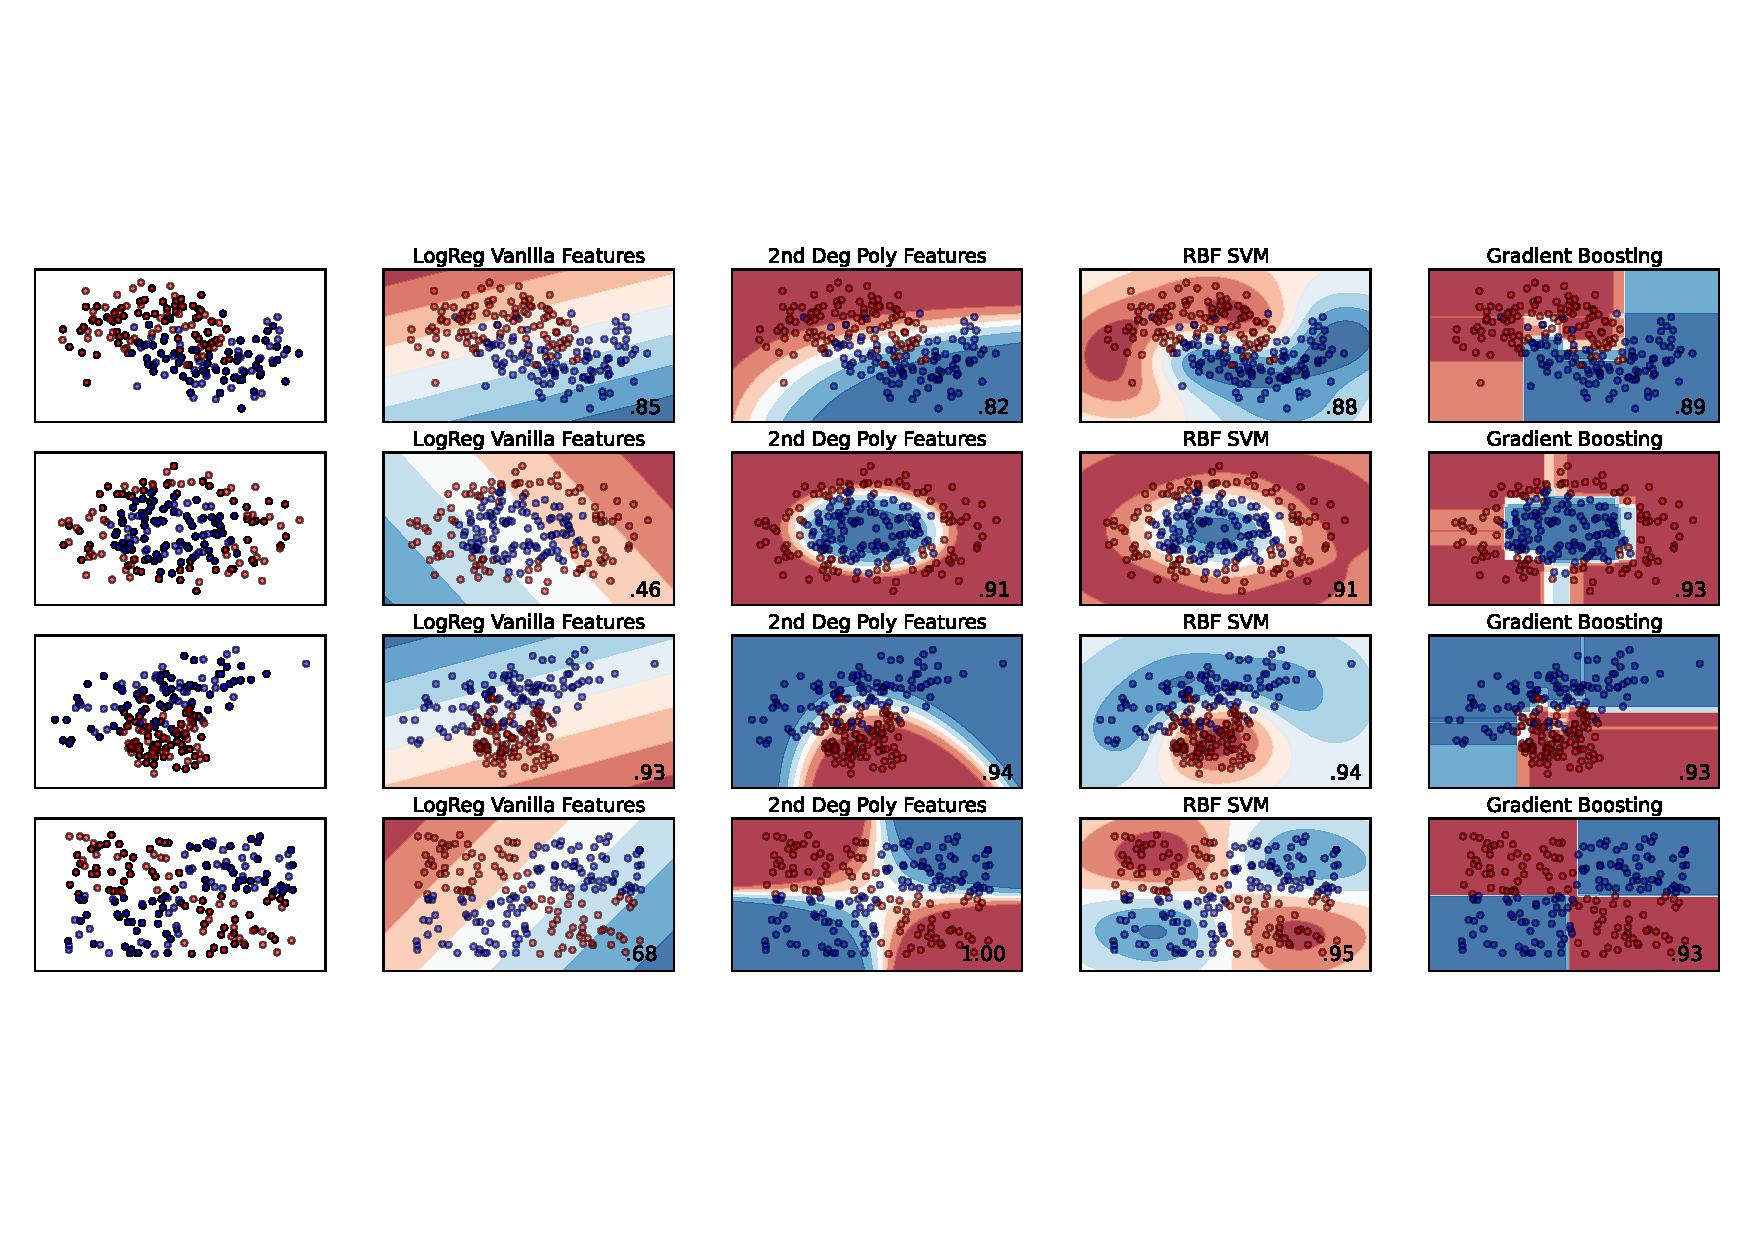
\includegraphics[scale=0.65]{classifier_boundaries.pdf}
%    \caption{Decision boundaries for four classifier types on four different datasets. The darker the color, the more certain the decision.
%             The plain dataset is shown in the first column. Each other column is a type of classifier applied to that dataset. The classifier
%             types are logistic regression, logistic regression with second degree polynomial features, RBF SVM, and gradient boosting with decision trees.
%             The accuracy of each model is shown in the bottom right corner of that model's subplot.}
%    \label{fig:boundaries}
%\end{sidewaysfigure}

With polynomial features added, a simple linear classifier is capable of drawing decision boundaries
that take on the form of arbitrary parabolas, hyperbolas, and elipses. Beyond classification, polynomial regression \cite{theoryoflinearmodels} is a staple regression method.
While polynomial features are a well known and used concept in machine learning (e.g. \cite{pavlidis2002learning, konidaris2009skill, wiesler2009investigations}) and work has been done to improve their utilization (e.g. \cite{pevckov2008minimal, huang2010predicting}), this is the first work that we know of that exploits matrix sparcity 
to improve the speed with which they are calculated and allows them to be calculated for a sparse matrix.


\section{Sparse Polynomial Features} \label{sec:sparse}
If the vectors of a feature matrix are sparse, many of these products of features will be
zero, and are therefore unnecessary to calculate if the matrix is stored in a sparse matrix 
data structure. If the density (the fraction of nonzero elements) of the matrix is $d$ where $0 \le d \le 1$,
the number of nonzero polynomial features is

\begin{equation*}
\binom{dD+2-1}{dD-1} = \frac{d^2D^2+dD}{2}
\end{equation*}

and if only they were calculated, the time complexity of generating polynomial features
for a matrix of size $N \times D$ is $O(Nd^2D^2)$, quadratically lower than calculating them via brute force.

The question then is how to devise an algorithm to calculate polynomial features for a vector $\vec{x}$ so that
only the nonzero elements of $\vec{x}$ are considered during the calculation process. Two main components are needed: (1) the ability to
quickly access only the nonzero elements of $\vec{x}$ and (2) The ability to know which polynomial feature column
the product of features with indices $a$ and $b$ should be stored in.

The first of these necessary components is obtained simply by using the appropriate data structure
to store the sparse matrix (e.g. storing it in compressed sparse row form). The second component 
is not only less readily available, but its necessity is less obvious. To make this need more clear, consider the
algorithm for the brute force calculation of polynomial features:

\begin{codebox}
\Procname{$\proc{Dense Polynomial Features}(A)$}
    \zi $N \gets$ row count of $A$
    \zi $D \gets$ column count of $A$
    \zi $B$ $\gets$ Matrix of size $N \times \frac{D^2+D}{2}$
    \zi \For $\id{row}$ in $A$ \Do
    \zi     $k \gets 0$
    \zi     \For $\i \gets 0 \To D$ \Do
    \zi         \For $\j \gets i \To D$ \Do
    \zi             $B[i, k] \gets \id{row}[i] \cdot \id{row}[j]$
    \zi             $k \gets k + 1$
                \End
            \End
       	\End
\end{codebox}

Notice that, for an individual row, the way the column the polynomial feature between features $i$ and $j$ can be determined
by a simple counter $k$ that is incremented each pass through the inner loop. This cannot be
done if we only calculate products between nonzero elements of $\vec{x}$, because all that
will be known is the nonzero element indices - many iterations will be skipped (hence the improved computational complexity).

What is therefore needed is a mapping between column index pairs of $\vec{x}$ and the space ${0, 1, ..., \frac{D^2+D}{2}-1}$
(the output size of second degree polynomial features when $D = |\vec{x}|$). The ordering of the mapping is irrelevant so long as its input 

\begin{equation*} \label{eq:input}
I \defeq \{(a, b) : a, b \in \{0,1,..., D-1\} \land a \le b\}
\end{equation*}

is bijective with its output

\begin{equation*} \label{eq:output}
O \defeq \{0, 1, ..., \frac{D^2+D}{2}-1\}
\end{equation*}

To construct this mapping, consider a matrix of size $D \times D$ where cell $(a,b)$ represents the
polynomial feature between indices $a$ and $b$ for $a,b \in I$ for vector $\vec{x}$.

\renewcommand{\kbldelim}{(}% Left delimiter
\renewcommand{\kbrdelim}{)}% Right delimiter
\[
  \kbordermatrix{
             & x_0    & x_1   & \cdot   & \cdot   &  \cdot  &  x_{D-1} \\
     x_0     & 0      & 1     & \cdot   &  \cdot  &  \cdot  &  D-1     \\
     x_1     & -      & D     & \cdot   &  \cdot  &  \cdot  &  2D-2    \\
     \cdot   & \cdot  & \cdot &  \cdot  &      &      &  \cdot       \\
     \cdot   & \cdot  &       &  \cdot  &  \cdot  &      &  \cdot       \\
     \cdot   & \cdot  &       &         &  \cdot  &  \cdot  &  \cdot       \\
    x_{D-1}  & -      & \cdot &  \cdot  & \cdot   & -    &  \frac{D^2+D}{2}-1\\
  }
\]

Again, any bijective mapping $I \mapsto O$ would suffice, but this particular mapping could
be considered one of the more natural options as it maps $I$ onto $O$ where both $I$ and $O$ are sorted in ascending order.
As can be seen, the required mapping can be viewed as mapping the upper triangular matrix (including 
the diagonal), whose indicies are $I$, onto $O$. The construction of this mapping will now
be given.

\newpage
INSERT JOHN'S PROOF HERE

The mapping can be modified slightly to yield interaction features instead of polynomial features
by noting that the section of the $D \times D$ mapping matrix that will yield interaction
features differs only in that its diagonal is excluded. The mapping is therefore gotten by
taking the polinomial mapping and subtracting $i+1$.

\newpage

\section{The Algorithm}
In section X we showed why a mapping from the space X
onto the space X is necessary for calculating polynomial features for a sparse matrix, then
derived such a mapping.

We now have the necessary components for an algorithm to efficiently calculate polynomial features for
a sparse matrix. The matrix needs to be stored in a form that allows for its nonzero column indices, e.g. in sparse row form,
and we will use the mapping derived in X to determine which column in the output space
the polynomial feature between two input columns is mapping onto. Combining these ideas yields the following algorithm:

\begin{codebox}
\Procname{$\proc{Sparse Polynomial Features}(A)$}
    \zi $\func{PolyMap}(a, b) = \frac{2Da-a^2+2b-3a-2}{2}+a+1$
    \zi $N \gets$ row count of $A$
    \zi $D \gets$ column count of $A$
    \zi $B$ $\gets$ Compressed Sparse Row Matrix of size $N \times \frac{D^2+D}{2}$
    \zi \For $\id{row}$ in $A$ \Do
    \zi     $N_{zc} \gets$ nonzero columns of $row$
    \zi     \For $i \gets 0 \To |N_{zc}|$ \Do
    \zi         \For $j \gets i \To |N_{zc}|$ \Do
    \zi             $k \gets \func{PolyMap}(i, j)$
    \zi             $r \gets$ index of $\id{row}$
    \zi             $B[r, k] \gets \id{row}[i] \cdot \id{row}[j]$
                \End
            \End
       	\End
\end{codebox}

Using the mapping for interaction features and changing the bounds in the loop conditions and the size of the output matrix, 
the algorithm can be modified to give second order interaction features:

\begin{codebox}
\Procname{$\proc{Sparse Interaction Features}(A)$}
    \zi $\func{InterMap}(a, b) = \frac{2Da-a^2+2b-3a-2}{2}$
    \zi $N \gets$ row count of $A$
    \zi $D \gets$ column count of $A$
    \zi $B$ $\gets$ Compressed Sparse Row Matrix of size $N \times \frac{D^2-D}{2}$
    \zi \For $\id{row}$ in $A$ \Do
    \zi     $N_{zc} \gets$ nonzero columns of $row$
    \zi     \For $i \gets 0 \To |N_{zc}|-1$ \Do
    \zi         \For $j \gets i+1 \To |N_{zc}|$ \Do
    \zi             $k \gets \func{InterMap}(i, j)$
    \zi             $r \gets$ index of $\id{row}$
    \zi             $B[r, k] \gets \id{row}[i] \cdot \id{row}[j]$
                \End
            \End
       	\End
\end{codebox}

where $N_{zc}$ are the columns of nonzero elements of row $\id{row}$.

\section{Analysis}

\subsection{Analytical}
We assume the input matrix $A$ is in sparse row form. The steps prior to the first loop are
constant operations. The outer loop will be executed $N$ times (once for each row). For each row, 
the innermost loop will be executed and the inner loop will be $\frac{|N_{zc}|^2+|N_{zc}|}{2}$ times.
If the density is uniformly distributed across all rows, $E[|N_{zc}|] = dD$, but this cannot be assumed. In the worst case,
then, the innermost loop will each be executed $\frac{D^2+D}{2}$ times, but on average, $\frac{d^2D^2+dD}{2}$ times.
The operations in the innermost loop are constant. The time complexity is therefore $O(ND^2)$ and $\Theta(Nd^2D^2)$.

It's often the case in a machine learning setting that the input matrix has near uniform density across its rows.
For example, if the matrix is sparse due to one-of-m encoding (also known as one-hot vectors), each row vector will
have the same number of nonzero components.

\subsection{Empirical}
To assess the performance of the algorithm on data of varied density, we compare its speed
to the PolynomialFeatures class of the popular machine learning scikit-learn \cite{scikit-learn}.
Uniformly random matrices of size $1000 \times D$ were generated for $d=0.2$, $0.4$, $0.6$, and $0.8$, and 
$D=1$, $101$, $201$, $301$, $401$, and $501$. Since the scikit-learn version of the algorithm
does not exploit sparsity, we assume the method's time is invariate with respect the density of the matrix, but
we gave it the lowest density of each dimensionality to be fair. The results are shown in figure \eqref{fig:benchmark}.

\begin{figure}
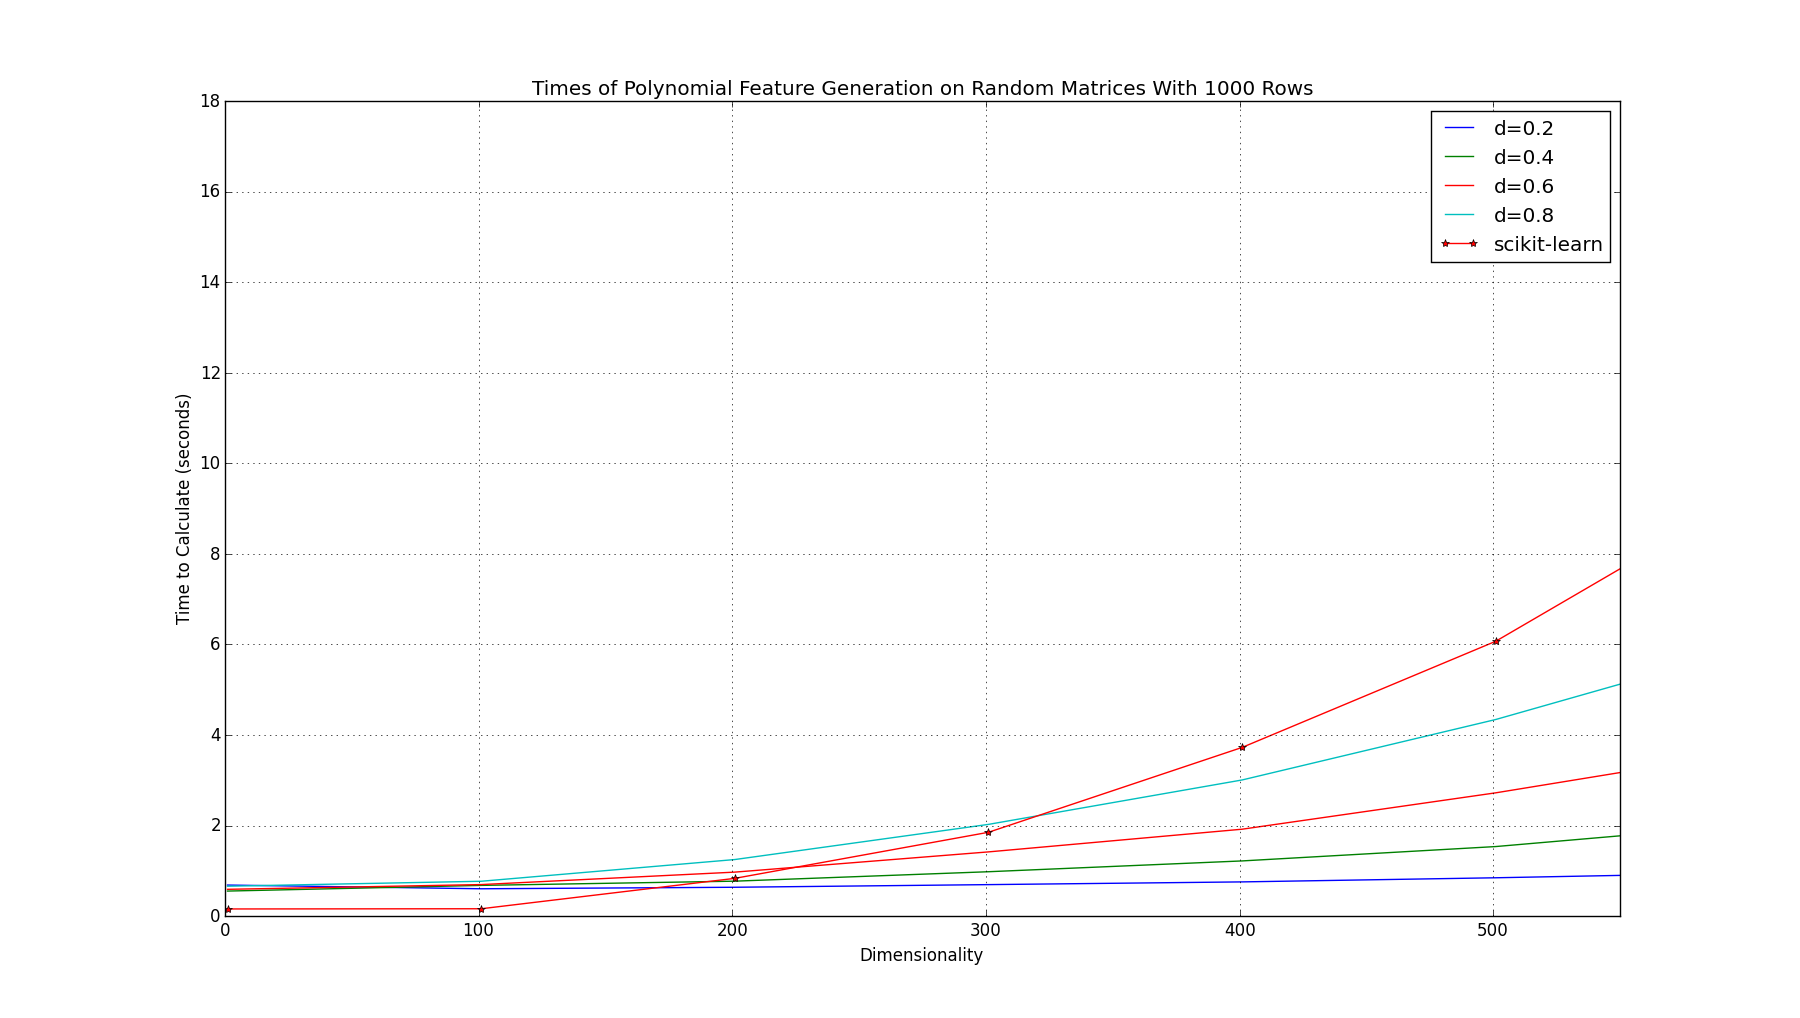
\includegraphics[scale=0.3]{benchmark_results.png}
\caption{This plot shows how long the sparse polynomial method took to run on matrices with 1000 rows of various dimensionalities and densities and compared to the scikit-learn PolynomialFeatures class on various dimensionalities.}
\label{fig:benchmark}
\centering
\end{figure}

As can be seen, the sparse method starts out slower than scikit-learn for each density. This
is either due to the overhead required by the sparse method (e.g. utilizing the mapping function),
or is due to implementation differences. The sparse method eventually becomes faster than scikit-learn
for each density. Note the excellent performance of $d=0.2$. This level of density is not uncommon when
working with sparse matrices.

The above benchmark was done on synthetic data. To more realistically determine the performance of
the algorithm, we applied it to two real world datasets: 20newsgroups\footnote{\url{http://scikit-learn.org/stable/datasets/twenty_newsgroups.html}} and connect-4, which was obtained
from the UCI Machine Learning Repository \cite{Lichman:2013}\footnote{\url{https://archive.ics.uci.edu/ml/datasets/Connect-4}}. We compare the time and space required by the sparse method and scikit-learn in table \eqref{table:results}.

\begin{center}
    \begin{tabular}{c | c | c} \label{table:results}
 %       \hline
        dataset             & 20newsgroups  & connect-4 \\ \hline
        instances           & 11,314        & 67,557    \\ \hline
        features            & 130,107       & 126       \\ \hline
        polynomial features & 8,463,980,778 & 8,127     \\ \hline
        density             & 0.12          & 0.11      \\ \hline
        dense space (MB)    & Memory Error  & 4191      \\ \hline
        sparse space (MB)   & 5333          & 735       \\ \hline
        dense time (s)      & Memory Error  & 26        \\ \hline
        sparse time (s)     & 109           & 44        \\ \hline
%        \hline
    \end{tabular}
\end{center}

Notice that scikit-learn was unable to calculate polynomial features for the 20newsgroups 
matrix; a memory error was encountered. The sparse method, however, succeeded in 109 seconds.
The resulting matrix had nearly 8.5 billion features. While most machine learning libraries would
struggle with such a high dimensionality, some, such as the system described in \cite{agarwal2014reliable} (which is 
available as part of the Vowpal Wabbit package\footnote{\url{https://github.com/JohnLangford/vowpal_wabbit/wiki}}), would likely be capable
of learning a model from such data.

The connect-4 dataset had its polynomial features computed faster via the dense method than the sparse. This
is likely because the dimensionality is sufficiently low for the overhead of the sparse method
to not have overtaken the dense method in terms of speed. However, the sparse method took less than
a fifth of the memory and took less than twice the speed, so using the sparse method during parameter 
optimization in a multi-core setting would drastically increase parameter search throughput.

\section{Summary \& Future Work}
In this work we have given a method of calculating second degree polynomial features on sparse matrices
with time complexity that quadratically decreases with respect to the density of the matrix.

This work also gives a general pattern for calculating polynomial features of arbitrary degrees:
instead of finding a mapping from the 2-tuples of indices onto the space $\{0, 1, ..., \frac{D^2+D}{2}-1\}$,
construct a mapping from k-tuples of indices onto the space $\{0, 1, ..., \binom{D+k-1}{D-1}-1\}$, where $k$ is the degree of the polynomial.
In terms of the upper triangular matrix analogy, this corresponds with mapping the upper k-simplex of a $(D, D, ..., D)$-tensor onto
the space $\{0, 1, ..., \binom{D+k-1}{D-1}-1\}$. For the average case of $dD$ nonzero elements per row, 
there will be $\binom{dD+k-1}{dD-1} = $ polynomial features, so the average time complexity for an $N \times D$ matrix
is $\Theta(Nd^kD^k)$, which means that its time complexity polynomially decreases with respect to the density
compared to the dense algorithm (which has $O(ND^k)$ and $\Theta(ND^k)$).

\vskip 0.2in
\bibliography{paper2}{}
\bibliographystyle{plain}
\end{document}